%% ─────────────────────────────────────────────────────────────────────────
%% gcrisk (repo: gcr-dosimetry-pipeline) — Life Sciences in Space Research submission
%% Built on Elsevier's cas-dc (double column) template.
%% ─────────────────────────────────────────────────────────────────────────

\documentclass[a4paper,fleqn]{cas-dc}

\usepackage[authoryear,longnamesfirst]{natbib}
\usepackage{mathtools}
\usepackage{siunitx}
\usepackage{verbatim}

% ── Custom commands ─────────────────────────────────────────────────────
\newcommand{\gcm}{\,\mathrm{g\,cm^{-2}}}
\newcommand{\mGyday}{\,\mathrm{mGy\,day^{-1}}}
\newcommand{\mSvday}{\,\mathrm{mSv\,day^{-1}}}
\newcommand{\keVum}{\,\mathrm{keV\,\mu m^{-1}}}
\newcommand{\Qeff}{Q_\mathrm{eff}}
\newcommand{\LETd}{\overline{L}_D}
\newcommand{\REID}{\mathrm{REID}}
\newcommand{\code}[1]{\texttt{#1}}

\begin{document}
\let\WriteBookmarks\relax
\def\floatpagepagefraction{1}
\def\textpagefraction{.001}

\shorttitle{Open-source GCR dosimetry pipeline for Mars mission risk}
\shortauthors{A.H.~Shah}

\title[mode=title]{An open-source GCR dosimetry pipeline for Mars mission
risk assessment: organ-specific REID, SEP acute hazard, and global
uncertainty quantification}

\author[1]{Aryan Hemendra Shah}[orcid=0009-0008-0518-428X]
\cormark[1]
\ead{ahs222@miami.edu}
\credit{Conceptualization, Methodology, Software, Validation, Formal
analysis, Investigation, Data curation, Writing -- original draft,
Writing -- review and editing, Visualization}

\affiliation[1]{organization={University of Miami},
            city={Miami},
            state={FL},
            country={USA}}

\cortext[1]{Corresponding author}

\begin{abstract}
I describe \textsc{gcrisk}, an open-source Python package
for estimating galactic cosmic ray (GCR) radiation exposure and cancer
risk on crewed deep-space missions. GCR flux, generated via force-field
solar modulation with inter-species composition constrained to ACE/CRIS
and PAMELA measurements, is transported through slab shielding via the
continuous-slowing-down approximation; organ-specific cancer risk (REID)
is estimated across eleven organs. A single global scale is fit to the
MSL/RAD cruise-phase absorbed dose ($1.84$~mGy/day at $16\gcm$ aluminum).
Independent checks (shielding-depth dependence, material ratio, real
MSL/RAD and ISS telemetry) agree within benchmark uncertainties;
day-to-day correlation against real telemetry is confounded by a documented
SEP event and is consistent with zero once it is excluded, but the
multi-month trend is consistent, including against eight years of
independent ISS data ($r=0.62$). A Solar Energetic Particle module
estimates acute organ dose for three historical events.

Global uncertainty is propagated via Latin Hypercube Sampling over nine
physics and radiobiological parameters, giving a median REID of
$6.5\%$ for a 35-year-old male on a 259-day Earth--Mars transit at
$16\gcm$ aluminum (p5--p95: $1.7$--$20.0\%$). Radiobiological parameters
dominate REID variance ($>\!85\%$) over GCR physics ($<\!15\%$). A
value-of-information sweep shows halving the ICRP-60 quality-factor
uncertainty alone would cut p95 REID by $33.5\%$, more than every physics
parameter combined. Sweeping launch date over two real solar
cycles (2003--2022) shows median REID varies $3.4\times$ from launch
timing alone. The composition-constrained HZE fraction ($13.0\%$ at
$16\gcm$ Al) is $1.7\times$ the NSRL reference, attributed to the absence
of nuclear fragmentation in the transport model; the pipeline's
$\Qeff=3.32$ is correspondingly $27\%$ above the MSL/RAD measured value.
Source code, tests, and validation data are freely available on GitHub.
\end{abstract}

\begin{highlights}
\item Open-source, pip-installable pipeline for GCR dose and cancer risk (REID).
\item Species composition constrained to real ACE/CRIS and PAMELA measurements.
\item Validated against real MSL/RAD and 8 years of independent ISS telemetry.
\item Value-of-information sweep ranks which uncertainty to reduce first.
\item Launch timing alone, across two real historical solar cycles, shifts mission cancer risk by a factor of 3.4x.
\end{highlights}

\begin{keywords}
galactic cosmic rays \sep Mars dosimetry \sep radiation risk \sep REID \sep
solar energetic particles \sep uncertainty quantification
\end{keywords}

\maketitle

% ─────────────────────────────────────────────────────────────────────────
\section{Introduction}
\label{sec:intro}

Deep-space human exploration beyond low-Earth orbit exposes crew members to
galactic cosmic rays (GCR) and solar energetic particles (SEP) at fluence
rates and energies far exceeding the shielding capacity of current crew
vehicles. GCR is the chronic, unavoidable component of this exposure and
sets the dose baseline for any multi-year mission, while SEP is episodic
but can deliver an acute dose in hours; this paper's pipeline centers on
the former, with a dedicated module for the latter (\S\ref{sec:sep_results}).
The GCR environment at 1--1.5~AU consists of protons, helium, and heavier
ions (the so-called HZE particles) spanning kinetic energies from a few
hundred MeV/n to tens of GeV/n. Biological effectiveness peaks near the
energy range where stopping power is highest.
A round-trip crewed Mars mission (transit + surface stay) of approximately
900 days is estimated to deliver a total effective dose of the order
$1$--$2$~Sv \citep{zeitlin2013}, which, depending on crew demographics and
the risk model used, implies a radiation-induced cancer mortality probability
that may approach or exceed NASA's career limit \citep{nasa2014}.

Quantifying that risk is not a single calculation: it requires combining
a calibrated, solar-modulation-responsive GCR spectral model, organ-resolved
dose transport, a cancer risk model accounting for HZE LET quality, and
uncertainty analysis that separates reducible physics uncertainty from the
larger radiobiological unknowns — and none of these combine trivially.
Tools such as HZETRN \citep{wilson1991}, OLTARIS, and Geant4/TOPAS each
address subsets of these requirements with greater physical rigor,
particularly nuclear fragmentation, but none is simultaneously openly
available, pip-installable, and integrated into one
uncertainty-quantified workflow: to my knowledge, no single open-source
tool combines GCR spectral modeling, organ-specific REID, SEP acute risk,
and global uncertainty propagation in one reproducible, pip-installable
workflow.

Here I present \code{gcrisk}, a Python package that,
within the limitations in \S\ref{sec:discuss_limits}: (1) generates
six-species GCR spectra with force-field modulation and ACE/CRIS/PAMELA-constrained
composition, calibrated to MSL/RAD; (2) transports spectra through slab
shielding via CSDA and nuclear attenuation with tabulated secondary
neutrons; (3) computes organ-specific dose and dose equivalent at eleven
ICRP-89 depths; (4) estimates REID via the Cucinotta (2013) EAR/ERR model;
(5) quantifies SEP acute BFO dose for three canonical events; and
(6) propagates global uncertainty via 9-parameter Latin Hypercube Sampling
with output variance decomposition.

The pipeline is not a replacement for HZETRN or Geant4 in high-fidelity
analysis. Its intended audience is mission designers, educators, and
researchers who need a transparent, reproducible, uncertainty-quantified
\emph{estimate} without standing up a closed high-fidelity code: the variance
decomposition — physics parameters together contribute $\sim\!12\%$ of
REID variance, radiobiological parameters $\sim\!88\%$ — and the
value-of-information and launch-window results below are difficult to
extract from existing closed tools.

% ─────────────────────────────────────────────────────────────────────────
% Methods — include detailed section from separate file

\section{Methods}
\label{sec:methods}

All computation is implemented in Python~3.9+ as the open-source package
\code{gcrisk}. The pipeline is a
sequence of composable modules: spectrum generation, slab transport, organ
dose, cancer risk (REID), SEP acute hazard, and uncertainty propagation, plus
a separate proton relative biological effectiveness (RBE) self-consistency
check. Full equations, parameter
tables, and derivations for every subsection below are given in
Supplementary Methods (Sections~S1.1--S1.9); only the essential physics and
the numbers needed to interpret the Results are summarized here.

\textbf{Trajectory and solar modulation.}
\label{sec:phi}
A Hohmann-transfer trajectory
(Earth 1.0~AU to Mars 1.524~AU, 259-day transit) sets the mission timeline.
Solar modulation potential $\phi(t)$ comes from the Usoskin et~al.\ monthly
reconstruction (real neutron-monitor data back to 1936); for the MSL transit
epoch, $\phi \approx 481\pm50$~MV. Neutron-monitor inter-station offsets
($\pm50$--$100$~MV) are propagated as an LHS parameter (\S\ref{sec:uq}).

\textbf{GCR spectrum.}
\label{sec:calib}
Solar modulation of GCR flux uses the Gleeson--Axford force-field
approximation applied to per-species local interstellar spectra (LIS):
protons and helium come from Vos \& Potgieter \cite{vos2015}, and C/O/Si/Fe from
the HelMod model of Boschini et al.\ \cite{boschini2020}. Inter-species
flux ratios are constrained to ACE/CRIS \citep{george2009} and PAMELA
\citep{adriani2014} measurements at the MSL epoch. A single global scale
is then fit to match the MSL/RAD absorbed dose of $1.84\mGyday$ at
$16\gcm$ aluminum \citep{zeitlin2013}. This is a one-free-parameter calibration
whose species mix is externally anchored, replacing an earlier
six-free-parameter fit with no compositional constraint. The resulting
HZE fraction ($13.0\%$ at $16\gcm$ Al) is $\sim\!1.7\times$ the NSRL
reference field \citep{slaba2016}, versus $\sim\!4\times$ under the prior
calibration; this residual excess is attributed to the CSDA transport
model not capturing nuclear fragmentation (Supplementary \S{}S1.3.3).

\textbf{Transport.} Ionization energy loss uses CSDA with Barkas
effective-charge scaling on NIST
PSTAR/ASTAR proton stopping powers. Nuclear interactions are modeled as
exponential fluence attenuation with a Bradt-Peters geometric mean free path
\citep{bradtpeters1950}, the same form underlying HZETRN's tabulated mean
free paths \citep{wilson1991}. This does not track secondary fragment
production, which is the model's primary physical limitation, most relevant
above $\sim\!30\gcm$ for Fe/Si. Secondary neutron dose equivalent uses a
pre-computed lookup calibrated to the HZETRN benchmark of Slaba et al.\
\cite{slaba2014} ($\pm25$--$30\%$, via LHS).

\textbf{Organ dose and quality factor.} Absorbed dose and ICRP-60 dose
equivalent \citep{icrp60} are computed at 11 organ-specific tissue depths
from ICRP Publication~89 \citep{icrp89}, weighted by ICRP-60 tissue factors.
The field effective quality factor is $\Qeff = \sum H_{k,s}/\sum D_{k,s}$
(numeric values and the ion-vs.-neutron breakdown: \S\ref{sec:let}).

\textbf{Cancer risk (REID).} REID is computed from the Cucinotta et al.\
\cite{cucinotta2013} organ-specific ERR/EAR model (NASA/TP-2013-217375),
using interpolated US sex-specific survival and baseline-mortality lookup
tables as a practical approximation to the full NASA/Cucinotta framework.
Point estimates use a fixed dose and dose-rate effectiveness factor
(DDREF) of $1.75$; the uncertainty ensemble
instead samples DDREF~$\sim$~Uniform$[1,2]$. REID's distribution is
right-skewed because \code{Q\_factor} (\S\ref{sec:uq}), the dominant tail
driver, is drawn from a heavy-tailed lognormal; the effective quality
factor is clipped at the ICRP-60 physical maximum of $30$, and the
resulting REID sample is separately clipped to $[0,1]$ since it represents
a probability (Supplementary \S{}S1.6).

\textbf{SEP acute risk.} Event fluence spectra use the Band function
\citep{tylka2006} for three canonical events (August~1972, October~2003,
January~2005; parameters in Supplementary Table~S3). BFO absorbed dose is
computed via CSDA transport through wall plus $10\gcm$ tissue and compared
to the NASA 30-day BFO limit of $250$~mGy \citep{cucinotta2010}. Mission SEP
encounter probability follows a Poisson process at solar-cycle-dependent
rates \citep{feynman1993}.

\subsection{Uncertainty Quantification}
\label{sec:uq}

Nine parameters are varied simultaneously via LHS: five physics
(solar modulation, LIS normalization, nuclear
cross-sections, neutron yield, HZE composition) and four biology (quality
factor scale, DDREF, ERR scale, EAR scale), each with a lognormal, uniform,
or clipped-normal prior justified by the relevant literature spread
(full distributions and justifications in Supplementary Table~S4). For each
LHS sample, a full mission dose integration is performed; publication
results use $N=500$ samples. Parameter sensitivity uses normalized
Spearman-$\rho^2$ decomposition (an approximation to first-order Sobol
indices).
\label{sec:sobol}

A separate value-of-information sweep (\S\ref{sec:vov}) re-runs the $N=500$
ensemble once per parameter, halving that parameter's prior spread while
holding all others at baseline, to quantify how much narrowing any one
source of uncertainty would actually reduce REID uncertainty
(\code{narrow} argument to \code{gcrisk.uncertainty.lhs\_samples}; Supplementary
\S{}S1.9).
\label{sec:vovmethod}

\subsection{Dose-Averaged LET and Proton RBE Self-Consistency Check}
\label{sec:letmethod}
\label{sec:rbemethods}

Per-species and field dose-averaged LET ($\overline{L}_D$) are computed to
trace $\Qeff$ to specific ion contributions (\S\ref{sec:let}; full
definitions in Supplementary \S{}S1.9). The same $\overline{L}_D$
infrastructure also implements two proton RBE models, Wedenberg et~al.\
(2013) \citep{wedenberg2013} and McNamara et~al.\ (2015)
\citep{mcnamara2015}, matched to OpenTOPAS-RBE scorer conventions and
checked only as an implementation self-consistency test
(Table~\ref{tab:validation}). This
layer is the foundation for a separate, planned proton-therapy crossover
study.


% ─────────────────────────────────────────────────────────────────────────
\section{Results}
\label{sec:results}

\subsection{Dose Rate Validation}
\label{sec:validation}

Two independent checks benchmark the pipeline against data not used in
calibration: the shielding curve shape stays within the HZETRN benchmark
envelope ($\lesssim20\%$) \citep{slaba2014} at $5$, $10$, and $30\gcm$
aluminum, and the Al/PE dose ratio ($1.36$) is consistent with Mrigakshi
(2013)'s $1.43\pm0.22$. As a separate internal self-consistency check
(not an external validation), the pipeline's own dose rate correlates with
its own $\phi$ input at $r=-0.998$ ($n=260$ days).

For an independent daily comparison I obtained real MSL/RAD cruise-phase
telemetry from NASA's PDS archive (MSL-M-RAD-3-RDR-V1.0; $218$ of $253$
cruise days; \url{scripts/fetch_real_rad_cruise_data.py}), replacing
the statistically-reconstructed proxy used in earlier drafts. Day-to-day
Pearson agreement over all 218 days is weak ($r=-0.127$, $p=0.06$), but this
is substantially an artifact of one real event: an X5.4 flare (AR11429) on
2012-03-07 produced one of the largest SEP events of solar cycle 24
($\sim\!6530$~pfu), and RAD's raw dose rate spikes $\sim\!30\times$ above
baseline the next day. Since this pipeline models SEP as a physically
separate, episodic module from chronic GCR (\S\ref{sec:sep_results}),
comparing the GCR-only daily model against telemetry containing a live SEP
spike is \emph{not a fair test} for those few days.

Two independent checks confirm the weak $r$ above is the outlier talking,
not a real signal being masked. \emph{Spearman's} $\rho$ (rank-based,
insensitive to a single large spike) on the \emph{full}, unmodified series
is already $\approx0$ ($\rho=-0.007$, $p=0.92$). And Pearson $r$ computed
with the documented event window excluded is also $\approx0$
($r=-0.001$, $p=0.99$, $n=209$) — note that $p$ \emph{rising} here, from
$0.06$ to $0.99$, is the expected direction, not a regression: a p-value
answers "how consistent is this $r$ with zero," and $r$ itself moved from
$-0.127$ toward $0$, so $p$ correctly moved toward $1$. There is no
cleaner signal hiding underneath the SEP day; removing it just removes
the one thing that was pulling $r$ away from zero. (I also tested whether
giving the model genuine daily-resolution modulation — a real Oulu
neutron-monitor daily count rate, calibrated to $\phi$ on an independent
1995--2011 window — would produce a real signal instead; it does not,
$r=-0.127\to-0.119$, ruling out "$\phi$ needs finer resolution" as an
explanation too.) Taken together, this is the honest ceiling for a
monthly-resolution force-field model against real telemetry that also
carries its own counting-statistics noise: no daily-resolution signal,
in either direction.

The multi-month trend the model \emph{is} built to capture is consistent in magnitude and direction
(real $+17.5\%$ vs.\ modeled $+14.5\%$, first-to-last cruise decile). Because
this RAD-anchoring is itself fit to the evaluated data, I additionally
tested generalization by splitting the series in half and fitting/testing
in both directions: held-out RMS error ($21.4\%$, $24.8\%$) is close to
in-sample RMS error ($23.5\%$, $19.4\%$) — a $5.5$-point maximum
degradation, showing the anchoring is not an artifact of testing on the
period it was fit to.

Table~\ref{tab:validation} summarizes all comparisons by epistemic
strength. The calibration-point dose rate ($1.843\mGyday$ vs.\ RAD's
$1.84\pm0.33$) is a direct consequence of fitting, not an independent
prediction.

\begin{table*}[t]
  \centering
  \caption{Pipeline benchmarks grouped by epistemic status:
           \textit{Independent} (not used in calibration),
           \textit{Calibration} ($\dot{D}$ fitted; $\dot{H}$, $\Qeff$ are
           predictions), \textit{Self-consistency} (no external reference).}
  \label{tab:validation}
  \small
  \begin{tabular*}{\tblwidth}{@{}LCCCC@{}}
    \toprule
    Quantity & Pipeline & Reference & Source & Rel.\ error \\
    \midrule
    \multicolumn{5}{l}{\textit{Independent benchmarks (not used in calibration)}} \\
    Shielding slope (5--30 g/cm²)
      & within & HZETRN env. & \cite{slaba2014} & $<20\%$ \\
    $\dot{D}$ ratio (Al vs PE, $16\gcm$)
      & 1.36  & $1.43\pm0.22$ & \cite{mrigakshi2013} & 5\%  \\
    Cruise trend (early vs.\ late decile)
      & $+14.5\%$ & $+17.5\%$ & NASA PDS RAD RDR & 3 pts \\
    Daily $r(\dot{D}_\mathrm{model}, \dot{D}_\mathrm{RAD})$, $n=218$
      & $-0.127$ & --- & NASA PDS RAD RDR & SEP-confounded, see \S\ref{sec:validation} \\
    Daily $r$, SEP window excl., $n=209$
      & $-0.001$ & --- & NASA PDS RAD RDR & $p=0.99$ \\
    Monthly $r$, ISS solar-cycle, $n=91$, 2010--18
      & $0.617$ & --- & ISS TEPC (CDAWeb) & $p=7\times10^{-11}$ \\
    \midrule
    \multicolumn{5}{l}{\textit{Calibration point ($\dot{D}$ fitted; $\dot{H}$ and $\Qeff$ are model predictions)}} \\
    $\dot{D}$ (mGy/day) at $16\gcm$ Al
      & 1.84  & $1.84\pm0.33$ & \cite{zeitlin2013} & $<1\%$ \\
    $\dot{H}$ (mSv/day) at $16\gcm$ Al
      & 6.09  & $4.81\pm0.97$ & \cite{zeitlin2013} & $+27\%$ \\
    $\Qeff$ at $16\gcm$ Al
      & 3.32  & $2.62\pm0.14$ & \cite{zeitlin2013} & $+27\%$ \\
    \midrule
    \multicolumn{5}{l}{\textit{Self-consistency (no external reference data)}} \\
    RBE (V79, Wedenberg)
      & 1.154  & 1.153  & TOPAS-nBio & $<10^{-3}$ \\
    RBE (V79, McNamara)
      & 1.165  & 1.165  & TOPAS-nBio & $<5\times10^{-8}$ \\
    Daily $r(\dot{D}, \phi)$, $n=260$
      & $-0.998$ & --- & --- & --- \\
    \bottomrule
  \end{tabular*}
\end{table*}

\subsection{Independent Multi-Year Solar-Cycle Cross-Check}
\label{sec:iss_crosscheck}

The MSL cruise window above is 253 days within a single solar cycle; as a
longer, independent cross-check of the force-field modulation physics
beyond that window, I compared the pipeline's
phi-driven predicted dose-equivalent rate at 1~AU against real ISS
radiation telemetry (\code{ISS\_DOSANL\_TEPC}, NASA Space Radiation
Analysis Group, via CDAWeb; \url{scripts/fetch_iss_tepc_data.py},
\url{scripts/compare_iss_solar_cycle.py}), May~2010--April~2018 —
a full solar cycle, $\sim\!12\times$ longer than the MSL window. Because
the ISS orbits inside Earth's magnetosphere (geomagnetic shielding this
pipeline does not model), absolute dose levels are not comparable; only
the modulation \emph{trend} is tested. Figure~\ref{fig:iss} shows both
monthly-median series (91 months, one instrument-gap outlier dropped):
$r=0.617$ ($p=7\times10^{-11}$), with both series declining toward the
2014 solar maximum and rising sharply through 2018.

\begin{figure*}[t]
  \centering
  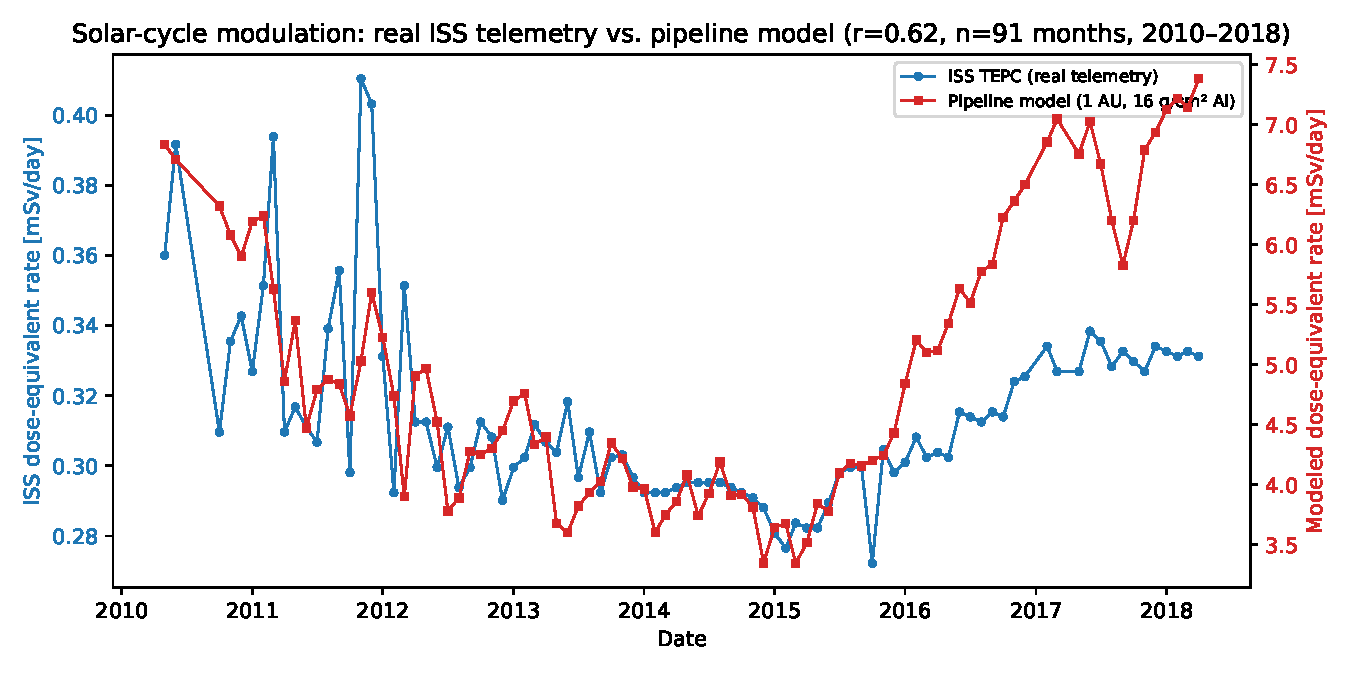
\includegraphics[width=0.85\textwidth]{figures/iss_solar_cycle.pdf}
  \caption{Real ISS TEPC telemetry (blue) vs.\ modeled dose-equivalent
    rate at 1~AU (red), May 2010--April 2018. Axes independently scaled
    (trend only, see text). $r=0.617$, $n=91$, $p=7\times10^{-11}$.}
  \label{fig:iss}
\end{figure*}

\subsection{Shielding Effectiveness and Uncertainty Bounds}
\label{sec:shielding_results}

Having validated the model's response to solar modulation, the next
question is how added shielding mass actually converts into dose.
Figure~\ref{fig:shielding_scan} shows absorbed dose rate vs.\ aluminum and
polyethylene shielding (259-day transit, $\phi=481$~MV) with p5--p95 LHS
bands. Dose decreases steeply to $\sim\!10\gcm$, then flattens above
$\sim\!16$--$20\gcm$ as secondary-neutron buildup offsets HZE attenuation;
the p5/p95 ratio at $16\gcm$ Al is $\sim\!1.9$ (dominated by LIS
normalization and neutron-yield uncertainty). Polyethylene gives
$\sim\!26\%$ lower dose than aluminum at $16\gcm$, consistent with
hydrogen-rich materials fragmenting HZE ions more effectively.

\begin{figure*}[t]
  \centering
  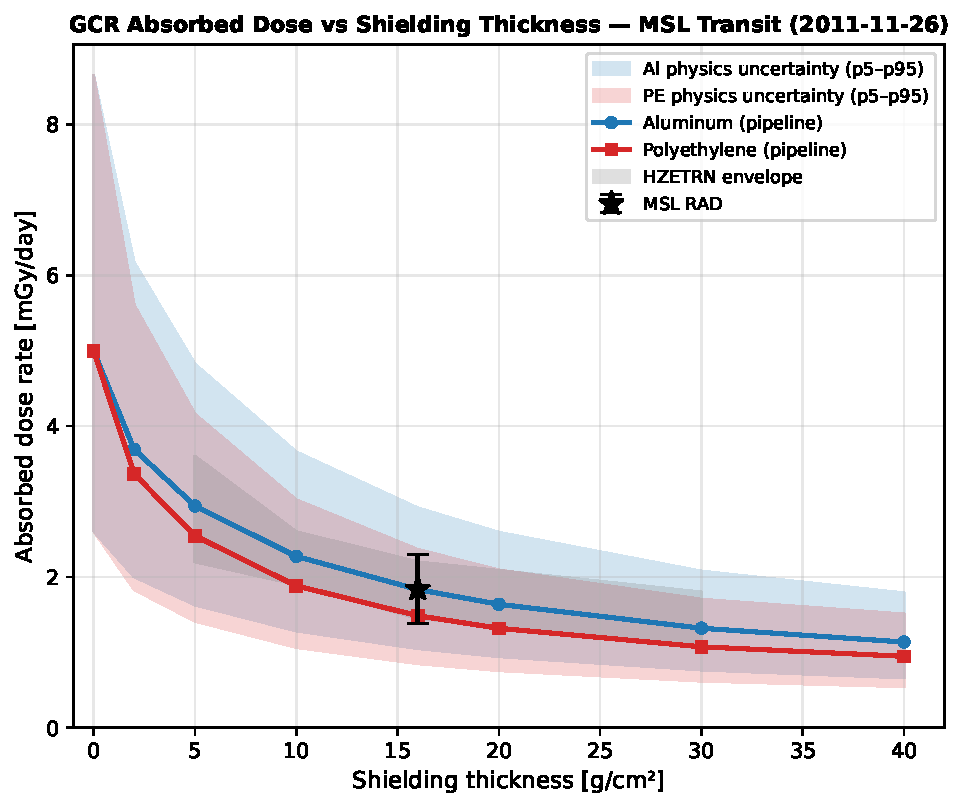
\includegraphics[width=0.7\textwidth]{figures/shielding_scan.pdf}
  \caption{Dose rate vs.\ Al/PE shielding with p5--p95 bands; MSL/RAD point
    (star); HZETRN envelope (gray).}
  \label{fig:shielding_scan}
\end{figure*}

The same shielding scan also shows which particles carry the dose at each
depth, in Figure~\ref{fig:species_fractions}. Protons dominate throughout
but their own fraction actually \emph{falls} with depth ($73.1\%\to68.9\%
\to58.0\%$ at $5$/$16$/$30\gcm$ Al), while carbon and oxygen's fractions
\emph{grow} ($3.8\%\to5.5\%\to8.0\%$ and $6.2\%\to6.7\%\to8.3\%$) even as
silicon and iron are attenuated toward zero ($<1.5\%$ by $5\gcm$, $<0.1\%$
by $30\gcm$). Since this transport model does not track nuclear
fragmentation (\S\ref{sec:discuss_limits}), this shift is each species'
own CSDA range-energy relationship playing out under increasing shielding,
not secondary production from the heavier ions: protons' steep,
low-energy-dominated spectrum is preferentially stopped as more material is
added, while carbon and oxygen's harder spectra let a larger share of their
own dose survive to greater depth.

\begin{figure*}[t]
  \centering
  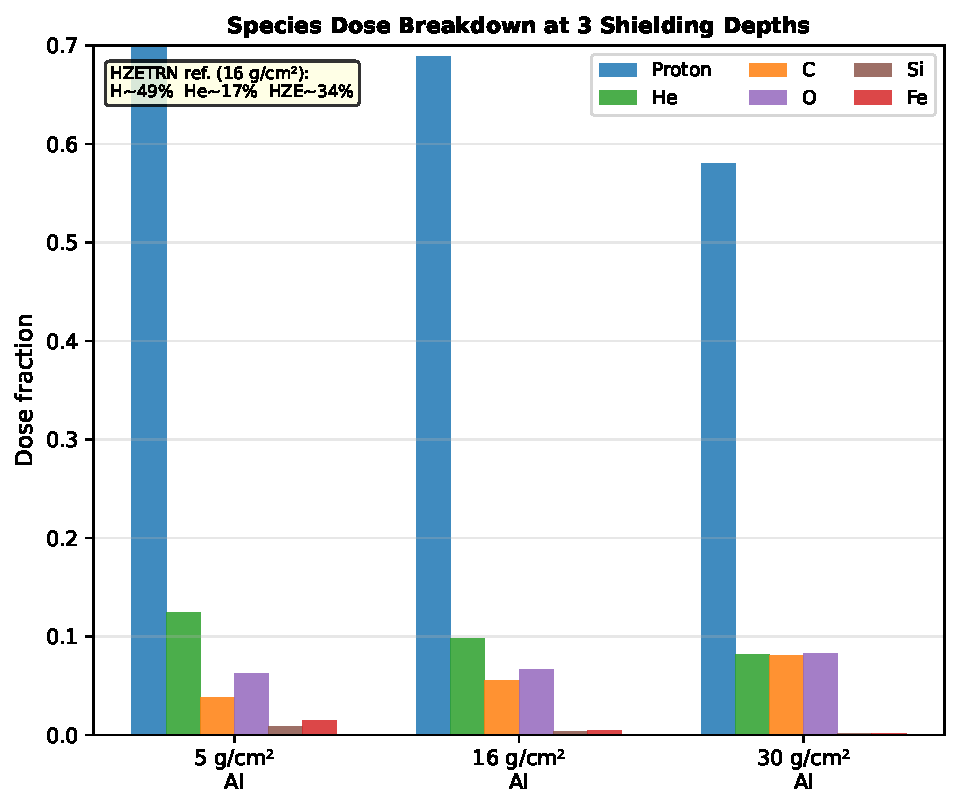
\includegraphics[width=0.7\textwidth]{figures/species_fractions.pdf}
  \caption{Per-species dose fractions at $5$, $16$, $30\gcm$ Al, with the
    HZETRN reference field's fractions at $16\gcm$ annotated for
    comparison.}
  \label{fig:species_fractions}
\end{figure*}

\subsection{Per-Species LET Decomposition}
\label{sec:let}

The plateau above $\sim\!16\gcm$ reflects a shift in which species carry
the dose, not a failure of shielding: Figure~\ref{fig:let} shows
dose-averaged LET per species and fractional
dose contributions at $0$, $16$, and $30\gcm$ aluminum. Unshielded at
$\phi=481$~MV, the HZE group ($Z>2$) is $20.9\%$ of absorbed dose (oxygen
$8.8\%$, iron $5.8\%$ dominant), consistent with GCR abundance ordering
and $Z^2$ stopping-power scaling; field $\LETd=3.9\keVum$ gives
$\Qeff^\mathrm{ions}=3.30$. After $16\gcm$ aluminum the HZE fraction falls
to $13.0\%$ (protons rise to $68.9\%$), field $\LETd$ drops to
$\sim\!2.5\keVum$, and the neutron contribution drives the total apparent
$\Qeff=3.32$ (\S\ref{sec:calib}).

\begin{figure*}[t]
  \centering
  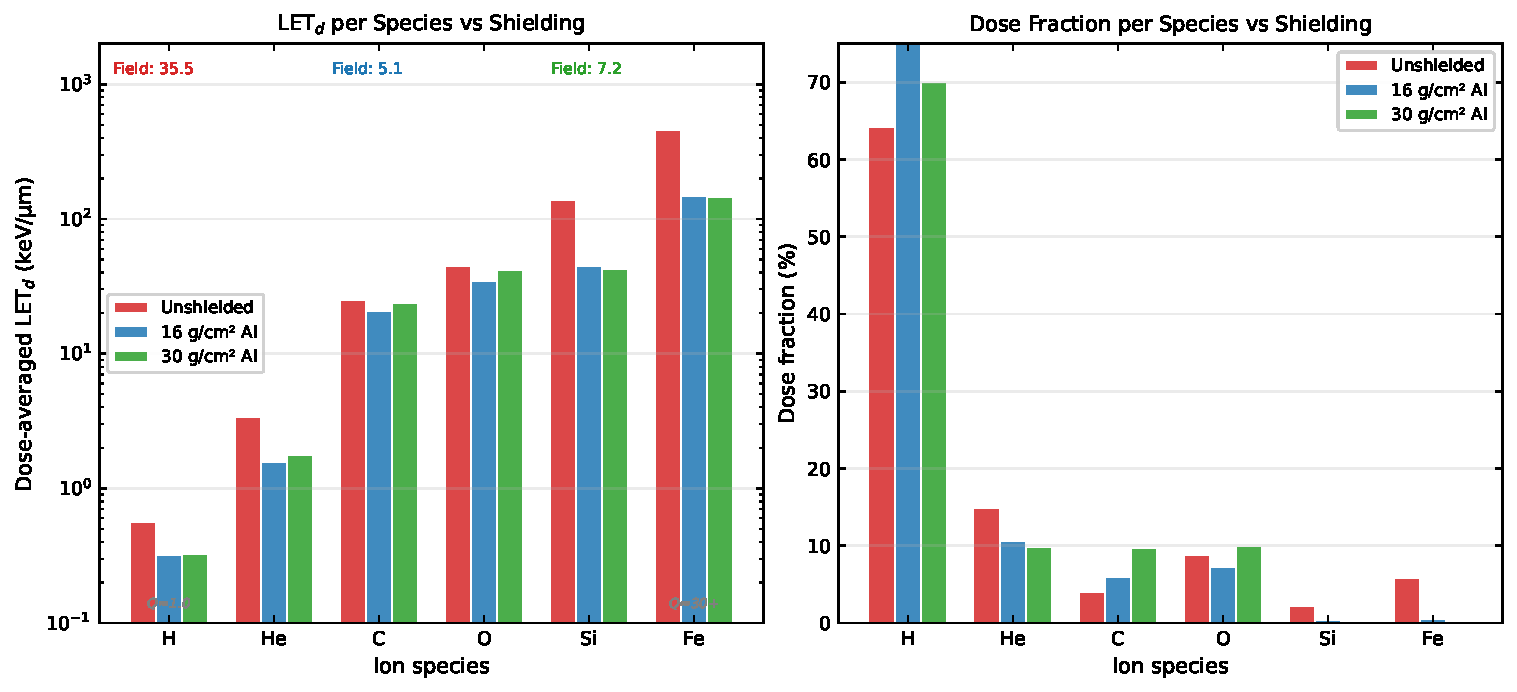
\includegraphics[width=0.85\textwidth]{figures/let_spectrum.pdf}
  \caption{Left: dose-averaged LET per species at 0, 16, 30 g/cm$^2$ Al.
    Right: fractional dose contribution per species; HZE fraction drops
    $20.9\%\to13.0\%$ as heavier ions attenuate preferentially.}
  \label{fig:let}
\end{figure*}

\subsection{SEP Acute Risk}
\label{sec:sep_results}

Chronic GCR exposure is only half the radiation picture; episodic SEP
events pose a distinct, acute hazard on the timescale of hours rather than
years. Figure~\ref{fig:sep} shows BFO absorbed dose from three canonical SEP
events vs.\ aluminum shielding. The August~1972 event delivers
$\sim\!37{,}000$~mGy unshielded ($\sim\!148\times$ the 30-day BFO limit of
250~mGy) and stays above the limit until $\sim\!32\gcm$; October~2003
needs $\sim\!25\gcm$; January~2005 falls below the limit under $20\gcm$.
GCR and SEP respond very differently to shielding: above $\sim\!20\gcm$,
added aluminum barely reduces chronic GCR dose but still substantially
cuts SEP dose. The August~1972 spectrum predates space-borne dosimetry
(reconstructed from ground-level neutron-monitor/riometry data
\citep{tylka2006}) and should be read as an order-of-magnitude estimate
($\sim\!\pm50\%$).

\begin{figure*}[t]
  \centering
  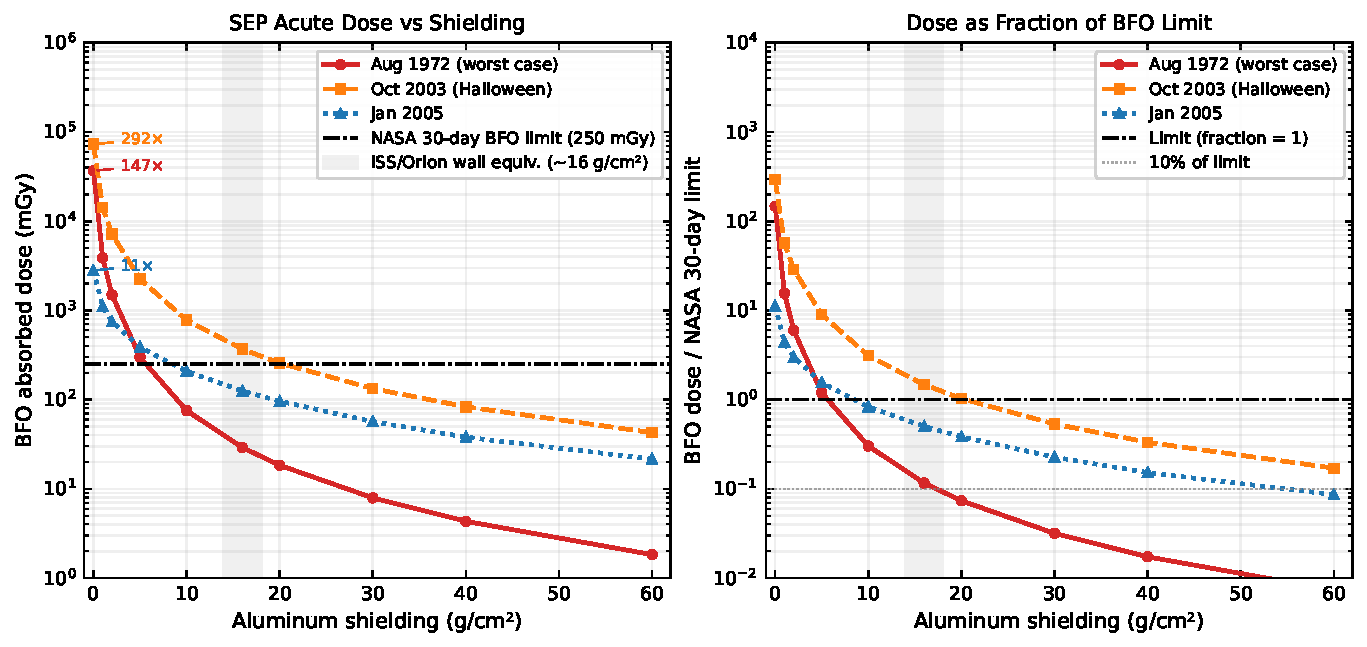
\includegraphics[width=0.85\textwidth]{figures/sep_shielding.pdf}
  \caption{Left: BFO dose (mGy) vs.\ Al shielding; line = NASA 30-day limit
    (250~mGy); band = ISS/Orion wall equivalent. Right: normalized to limit.}
  \label{fig:sep}
\end{figure*}

\subsection{REID vs.\ Shielding and Organ Contributions}
\label{sec:reid_results}

Returning to the chronic GCR side, the quantity mission planners ultimately
care about is not dose but cancer risk. Figure~\ref{fig:reid} shows REID
vs.\ aluminum shielding for a 35-year-old
male and female on a 259-day transit. At $16\gcm$, median REID is $6.5\%$
(male) and $8.3\%$ (female) — both above the historical NASA $3\%$ career
limit \citep{nasa2014}; the female excess reflects higher sex-specific
lung/breast ERR-EAR coefficients \citep{cucinotta2013}. p5--p95 bands
($1.7$--$20.0\%$ male, $2.2$--$25.7\%$ female) reflect the dominant
radiobiological uncertainty (\S\ref{sec:uq}): the mission is likely to
carry meaningful cancer risk, but the precise value is not resolvable
within the current radiobiological framework. Stomach, colon, and lung
contribute most to organ dose equivalent, consistent with their high
ICRP-60 weighting ($w_T=0.12$).

\begin{figure*}[t]
  \centering
  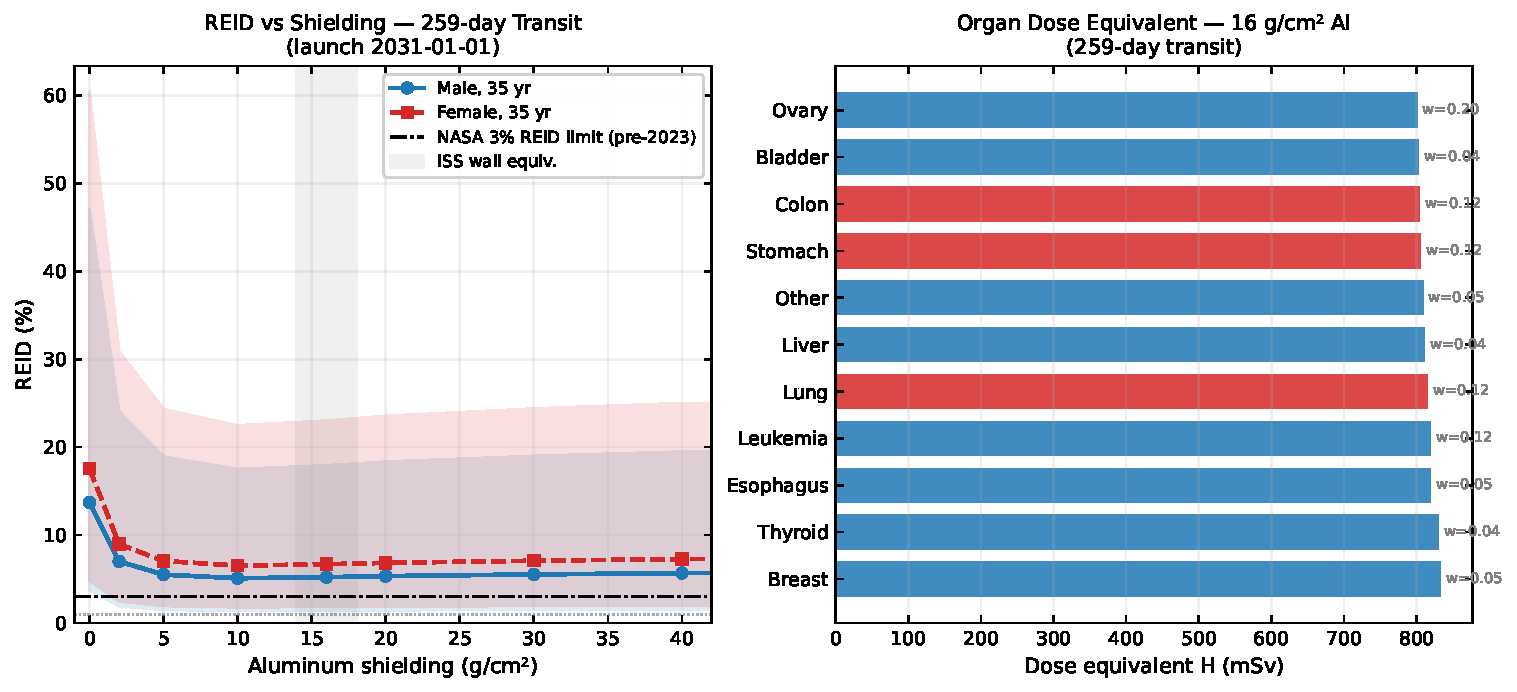
\includegraphics[width=0.85\textwidth]{figures/reid_shielding.pdf}
  \caption{Left: REID (\%) vs.\ Al shielding, male/female, p5--p95 bands;
    line = NASA 3\% limit. p95 at $<5\gcm$ exceeds physically meaningful
    values (LHS not clipped); $>10\gcm$ is more reliable. Right: organ
    dose equivalent at $16\gcm$ Al, $w_T$ annotated.}
  \label{fig:reid}
\end{figure*}

\subsection{REID vs.\ Launch Date Across the Solar Cycle}
\label{sec:launchwindow}

REID depends strongly on the solar modulation potential $\phi$ at launch.
I swept \code{gcr.reid.reid\_vs\_launch\_date} over monthly launch dates
(\url{scripts/launch_window_sweep.py}); Figure~\ref{fig:launchwindow}
separates two regions. The solid curve (2003--2022) uses real Usoskin
$\phi$ data spanning two full solar cycles; median REID ranges from
$3.3\%$ (May 2003, solar maximum, $\phi\approx853$~MV) to $11.3\%$ (May
2009, solar minimum, $\phi\approx388$~MV) — a $3.4\times$ spread from
launch timing alone, at fixed shielding and demographics. The dashed,
hatched curve (2023--2035) is \emph{not} database-derived: it is a
self-generated idealized $\sim\!11$-year cosine cycle, included only to
illustrate the qualitative shape a tool like this could show for a
future window \emph{if} the cycle repeats its characteristic period — not
a space-weather forecast, and not used to name a recommended future
launch date. Real cycles vary in amplitude and length by years; an
operational decision would need an actual forecast, outside this paper's
scope.

\begin{figure*}[t]
  \centering
  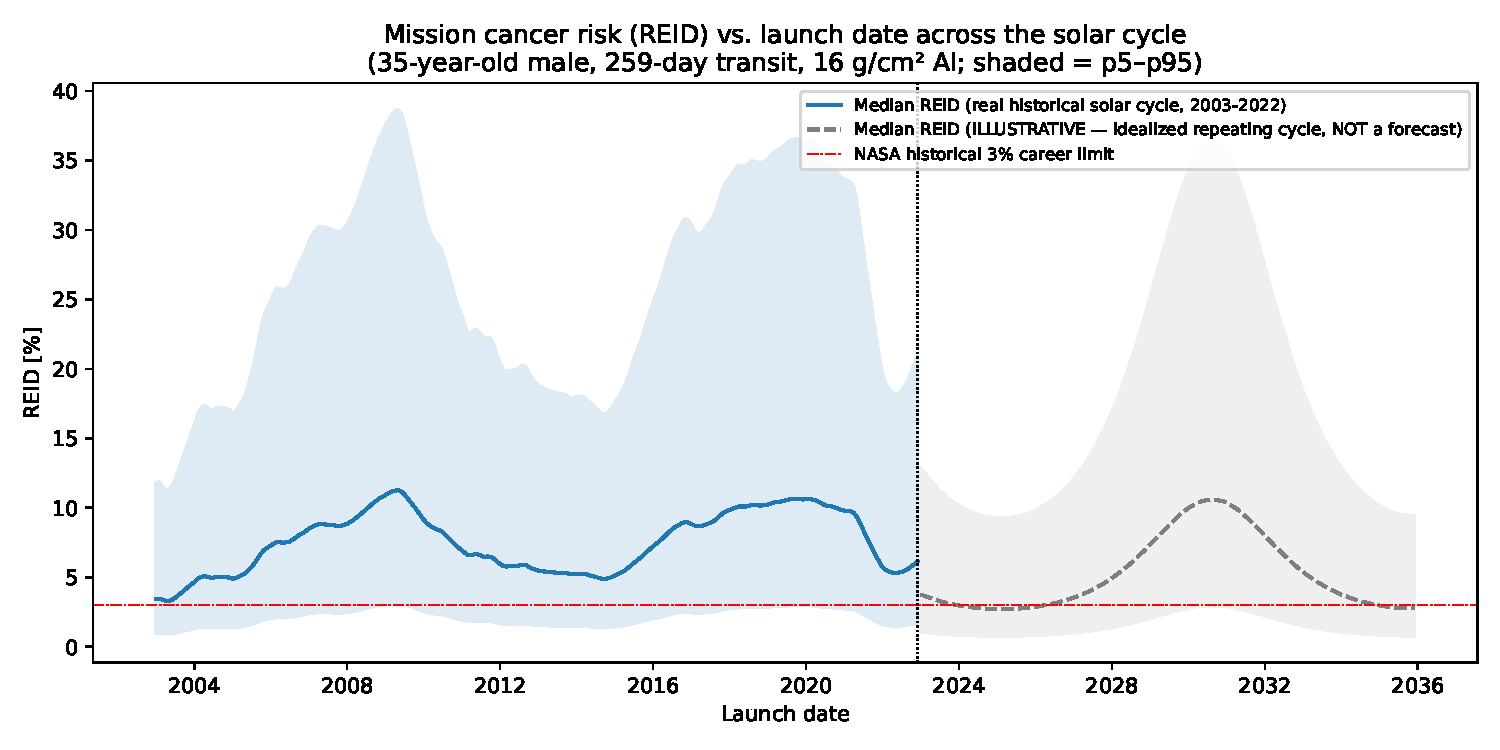
\includegraphics[width=0.85\textwidth]{figures/launch_window_sweep.pdf}
  \caption{REID vs.\ launch date (male, $16\gcm$ Al; shaded = p5--p95).
    Solid blue: real historical $\phi$ (2003--2022). Dashed/hatched: an
    idealized repeating cycle, \emph{not} a forecast (see text). Line =
    NASA 3\% limit.}
  \label{fig:launchwindow}
\end{figure*}

\subsection{Value of Narrowing Individual Uncertainty Parameters}
\label{sec:vov}

Launch timing is a free lever available at zero engineering cost; tightening
a physical or biological parameter is not, so the natural next question is
which parameter is worth that investment. The variance decomposition
(\S\ref{sec:sobol}) ranks parameters by their
share of REID variance under \emph{current} priors, but not how much
narrowing any one would help. I re-ran the $N=500$ ensemble once per
parameter, halving its uncertainty while holding the rest at baseline
(\url{scripts/sensitivity_narrowing_sweep.py}); Table~\ref{tab:vov}
ranks the resulting p95 REID reduction. Halving \code{Q\_factor} alone
shrinks p95 REID from $20.0\%$ to $13.3\%$ ($33.5\%$ reduction) —
$\sim\!7\times$ more than the next parameter (\code{DDREF}, $4.5\%$) and
more than every GCR physics parameter combined ($<5\%$). This makes
\emph{biology dominates} concrete: tightening the ICRP-60 quality-factor-model
uncertainty (e.g.\ expert elicitation or a track-structure-resolved
$Q(L)$ for mixed GCR fields) would narrow Mars mission REID uncertainty
more than every other parameter here combined.

\begin{table}[t]
  \centering
  \caption{Value-of-information sweep: reduction in p95 REID from halving
           one parameter's uncertainty at a time (35-year-old male,
           259-day transit, $16\gcm$ Al; baseline p95 $=20.0\%$).}
  \label{tab:vov}
  \small
  \begin{tabular*}{\tblwidth}{@{}LCCC@{}}
    \toprule
    Parameter & Narrowed p95 & $\Delta$ p95 & \% of baseline \\
    \midrule
    \code{Q\_factor}       & 13.3\% & $-$6.7 pts & $-$33.5\% \\
    \code{DDREF}           & 19.1\% & $-$0.9 pts & $-$4.5\%  \\
    \code{phi\_scale}      & 19.5\% & $-$0.5 pts & $-$2.7\%  \\
    \code{ERR\_scale}      & 19.8\% & $-$0.3 pts & $-$1.3\%  \\
    \code{LIS\_norm}       & 19.8\% & $-$0.2 pts & $-$1.1\%  \\
    \code{hze\_norm\_scale}& 19.9\% & $-$0.2 pts & $-$0.8\%  \\
    \code{neutron\_H}      & 20.0\% & $-$0.1 pts & $-$0.3\%  \\
    \code{EAR\_scale}      & 20.0\% & $-$0.0 pts & $-$0.1\%  \\
    \code{cross\_sec}      & 20.0\% & $0.0$ pts  & $0.0\%$   \\
    \bottomrule
  \end{tabular*}
\end{table}

% ─────────────────────────────────────────────────────────────────────────
% Discussion — include from separate file
% ─────────────────────────────────────────────────────────────────────────────
% DISCUSSION (condensed — extended limitations in Supplementary Material)
% ─────────────────────────────────────────────────────────────────────────────

\section{Discussion}
\label{sec:discussion}

\subsection{What the Validation Does and Does Not Show}
\label{sec:discuss_validation}

The independent checks in \S\ref{sec:validation}--\ref{sec:iss_crosscheck}
(shielding curve shape, material ratio, the real MSL/RAD cruise trend, and
the real ISS multi-year trend) each probe an aspect of the model not
constrained by the single-point MSL/RAD calibration. Together they support
characterizing the pipeline as \emph{calibrated to one flight measurement
and consistent with independent benchmarks within their stated
uncertainties}. The
near-zero daily-resolution correlation, the SEP-event confound behind it,
and the held-out cross-validation of the RAD anchoring (\S\ref{sec:validation})
are reported for the same reason: an honest, non-circular account of what
this monthly-resolution model can and cannot claim is worth more than an
artificially strong number. That discipline paid off here: chasing the
daily correlation initially suggested a resolution gap in the solar-modulation
physics, but a genuine daily-resolution reconstruction (real neutron-monitor
data, independently calibrated) did not improve it, and the actual
explanation turned out to be a documented SEP event contaminating the
comparison for a few days.

\subsection{Implications for Mission Shielding Design}
\label{sec:discuss_shielding}

Turning from validation to what these numbers imply operationally, the
shielding curve (Fig.~\ref{fig:shielding_scan}) plateaus above
$\sim\!20\gcm$ aluminum as secondary-neutron growth offsets HZE
attenuation: going from $16$ to $40\gcm$ cuts GCR dose only
$\sim\!42\%$ while roughly doubling wall mass, consistent with prior
literature \citep{cucinotta2006, slaba2014} that bulk aluminum shielding
is mass-inefficient against chronic GCR. SEP shielding is the opposite
case: the October~2003 event drops from $\sim\!35\times$ the BFO limit
unshielded to below it by $\sim\!25\gcm$ (Fig.~\ref{fig:sep}). This
asymmetry supports a compact, heavily-shielded SEP storm shelter over
whole-vehicle HZE shielding as the more mass-efficient architecture
\citep{durante2011, cucinotta2010}.

\subsection{REID Interpretation: Biology Dominates}
\label{sec:discuss_reid}

The shielding trade-offs above are only as meaningful as the risk number
they are designed around, so it is worth scrutinizing that number directly.
Median REID ($6.5\%$ male, $8.3\%$ female at $16\gcm$) exceeds the
historical NASA $3\%$ limit \citep{nasa2014}, though NASA's updated
age/sex-dependent framework \citep{nasa2023} is not implemented here and
the comparison should be read as indicative. Because the
composition-constrained pipeline overestimates $\Qeff$ by $\sim\!27\%$
(\S\ref{sec:calib}), these values are conservative upper estimates;
correcting for that ratio would put male median REID at $\sim\!5.1\%$ —
still above the historical limit. The p5--p95 band spans a factor of
$\sim\!12\times$: this REID should be read as "the mission dose likely
carries meaningful cancer risk, with the exact value uncertain by an
order of magnitude."

Most importantly, this uncertainty is overwhelmingly biological. The four
radiobiological parameters contribute $\gtrsim\!85\%$ of REID's normalized
sensitivity, all five physics parameters combined $<15\%$ (Supplementary
Table~S4) — consistent with Cucinotta et al.\ \cite{cucinotta2013} and the
broader literature \citep{durante2011}. No direct human data constrain the
HZE LET range that dominates unshielded GCR dose equivalent; extrapolating
from mouse and atomic-bomb-survivor data to this regime is the single
largest source of uncertainty in this calculation, and no amount of
improved transport physics can resolve it. Strikingly, \code{phi\_scale}
drives $79\%$ of absorbed-dose variance but only $8\%$ of REID variance:
solar-modulation uncertainty strongly affects physical dose but has almost
no leverage on mortality probability once biology enters. The
value-of-information sweep (\S\ref{sec:vov}) makes this actionable rather
than qualitative.

\subsection{Scope of the LET/RBE Layer}

Separately from the REID interpretation above, it is worth being explicit
about what the pipeline's LET/RBE layer does and does not claim. The
per-species LET decomposition (Fig.~\ref{fig:let}) traces $\Qeff$'s
physical origin to specific ion contributions; the residual $27\%$
$\Qeff$ excess over the RAD measurement is attributed to CSDA's missing
fragmentation (\S\ref{sec:calib}). The repository also contains a proton
RBE self-consistency layer (\S\ref{sec:rbemethods}) reported only as an
implementation check (Table~\ref{tab:validation}); it is the foundation
for a planned, separate proton-therapy crossover study.

\subsection{Limitations}
\label{sec:discuss_limits}

The main structural limitation is CSDA transport without nuclear
fragmentation, which by my order-of-magnitude estimate overestimates
$\Qeff$ (and correspondingly REID) at $16\gcm$ by roughly
$15$--$25\%$ \citep{wilson1991, slaba2014} — well within the $12\times$
uncertainty band but not negligible relative to the median. Other
significant approximations include: a uniform-slab spacecraft geometry
(no ray-tracing); six modeled GCR species (unmodeled species $<5\%$ of
dose); the force-field modulation's monthly resolution, which limits
daily-scale claims and is the reason the ISS cross-check is restricted to
trend and does not extend to near-Earth or trapped-radiation
environments; the pre-2023 Cucinotta NASA risk framework rather than the
updated age/sex-dependent limits; and cancer-only risk (no CNS,
cataract, or cardiovascular endpoints). The full itemized discussion of
each limitation, with supporting estimates, is provided in Supplementary
\S{}S2.

\subsection{Future Work}
\label{sec:future_work}

Each limitation above points to a concrete next step, roughly in order of
expected impact on REID. \textbf{Nuclear fragmentation}: replacing the
Bradt-Peters fluence-removal model with tabulated fragmentation
cross-sections \citep{wilson1991} would let secondary light-ion production
be tracked explicitly, closing the $15$--$25\%$ $\Qeff$ overestimate
(\S\ref{sec:discuss_limits}) rather than only bounding it. \textbf{Risk
framework}: adopting NASA's 2023 age/sex-dependent career-limit framework
\citep{nasa2023} in place of the pre-2023 Cucinotta model would remove the
main caveat on the REID-vs-NASA-limit comparison in
\S\ref{sec:discuss_reid}. \textbf{Geometry}: ray-traced, non-uniform
spacecraft shielding (as in OLTARIS or Geant4) would replace the
uniform-slab approximation, most relevant for real vehicle interiors with
mass concentrated unevenly around the crew. \textbf{Non-cancer endpoints}:
CNS, cataract, and cardiovascular risk models are not yet implemented; CNS
effects in particular have rodent-study support for a cognitive-impairment
threshold below the cancer risk threshold modeled here. \textbf{Proton
RBE}: the dose-averaged LET/RBE self-consistency layer
(\S\ref{sec:rbemethods}) exists as the foundation for a planned, separate
proton-therapy crossover study.

\subsection{Comparison with Existing Tools and Reproducibility}
\label{sec:discuss_comparison}

Set against the alternatives, Table~\ref{tab:tool_comparison} compares
this pipeline against HZETRN, OLTARIS, Geant4, and TOPAS: it trades
high-fidelity transport physics for being, to my knowledge, the only
one that is simultaneously open/pip-installable and includes
organ-specific REID, an SEP library, and LHS uncertainty quantification.

\begin{table}[t]
  \centering
  \caption{Comparison of GCR dosimetry tools. \checkmark\ = present,
           $\triangle$ = partial, $\times$ = absent.}
  \label{tab:tool_comparison}
  \small
  \setlength{\tabcolsep}{4pt}
  \begin{tabular*}{\tblwidth}{@{}lccccc@{}}
    \toprule
    Feature & Ours & HZETRN & OLTARIS & Geant4 & TOPAS \\
    \midrule
    Open / pip-install   & \checkmark & $\times$    & $\times$    & \checkmark  & \checkmark \\
    Fragmentation        & $\times$   & \checkmark  & \checkmark  & \checkmark  & \checkmark \\
    Organ REID           & \checkmark & $\triangle$ & \checkmark  & $\times$    & $\times$   \\
    SEP library          & \checkmark & $\triangle$ & \checkmark  & $\times$    & $\times$   \\
    LHS uncertainty      & \checkmark & $\times$    & $\times$    & $\times$    & $\times$   \\
    Clinical RBE         & \checkmark & $\times$    & $\times$    & $\triangle$ & \checkmark \\
    CI test suite        & \checkmark & $\times$    & $\times$    & $\times$    & $\times$   \\
    \bottomrule
  \end{tabular*}
\end{table}

All results reproduce via \texttt{pip install -e .[dev]},
\texttt{validate\_pipeline.py}, \texttt{validate\_extended.py}, and
\texttt{pytest}; the full $N=500$ ensemble takes $\sim\!90$ minutes
single-core, with a reduced $N=20$ path used in CI. No proprietary
datasets are required.


% ─────────────────────────────────────────────────────────────────────────
\section{Conclusion}
\label{sec:conclusion}

I have presented \textsc{gcrisk}, an open-source,
pip-installable Python package integrating GCR spectrum generation, CSDA
transport, organ-specific REID, SEP acute dosimetry, and LHS uncertainty
propagation, calibrated to MSL/RAD and consistent with HZETRN benchmarks
within stated uncertainties. Median REID at $16\gcm$ Al on a 259-day
transit is $6.5\%$ (p5--p95 $1.7$--$20.0\%$), above the NASA $3\%$ limit;
the wide band is dominated by biology, not GCR transport physics. On the
acute side, the August~1972 SEP event requires $>30\gcm$ Al for sub-limit
BFO protection, and at the $16\gcm$ reference geometry its dose is
$\sim\!4\times$ the limit. The HZE group ($Z>2$) accounts for $20.9\%$ of
unshielded dose ($\LETd=3.9\keVum$), falling to $13.0\%$ at $16\gcm$ Al,
and the model's solar-modulation trend independently tracks 8 years of
real ISS telemetry across a full solar cycle ($r=0.62$, $p=7\times10^{-11}$,
$n=91$) — a longer, separately-sourced cross-check than the MSL
calibration window it was fit to. Two results point toward what would
most improve the estimate: halving \code{Q\_factor} uncertainty alone cuts
p95 REID by $33.5\%$, $\sim\!7\times$ more than any other parameter or all
physics parameters combined (\S\ref{sec:vov}), identifying where research
investment matters most; and launch timing alone, over two real historical
solar cycles (2003--2022), swings median REID $3.4\times$
(\S\ref{sec:launchwindow}) at zero engineering cost.

All source code, 86 automated tests, and validation datasets are available
at \url{https://github.com/aryanhshah8/gcr-dosimetry-pipeline}.

% ─────────────────────────────────────────────────────────────────────────
\section*{Acknowledgements}

The author thanks the MSL/RAD team (C.~Zeitlin and collaborators) for making
the cruise-phase dosimetry data publicly available, without which calibration
of the pipeline would not have been possible, and NASA's Planetary Data
System (PDS PPI Node, dataset MSL-M-RAD-3-RDR-V1.0, producer S.~Rafkin) for
archiving the daily cruise-phase telemetry used in the independent
day-by-day comparison in Section~\ref{sec:validation}, and the NASA Space
Radiation Analysis Group (dataset ISS\_DOSANL\_TEPC, via NASA's CDAWeb)
for the ISS radiation telemetry used in the multi-year solar-cycle
cross-check (Section~\ref{sec:iss_crosscheck}).
The Usoskin et~al.\ solar modulation potential database, the Vos \&
Potgieter LIS parametrizations, and the HZETRN benchmark datasets of
Slaba et~al.\ are gratefully acknowledged.

% ─────────────────────────────────────────────────────────────────────────
\section*{Declaration of Competing Interests}

The author declares no competing interests.

% ─────────────────────────────────────────────────────────────────────────
\section*{Funding}

This research did not receive any specific grant from funding agencies in
the public, commercial, or not-for-profit sectors.

% ─────────────────────────────────────────────────────────────────────────
\section*{Data Availability Statement}

All source code, input datasets, validation scripts, and TOPAS benchmark
geometry files are freely available at
\url{https://github.com/aryanhshah8/gcr-dosimetry-pipeline}.
Full methods derivations, extended parameter tables, and extended
limitations discussion are provided as Supplementary Material.
No proprietary datasets were used; all input data (Usoskin solar
modulation potential database, NIST stopping powers, real MSL/RAD
cruise-phase dosimetry from NASA's PDS archive, and real ISS TEPC
telemetry from NASA's CDAWeb) are included in the repository under
\code{data/}, and the HZETRN neutron benchmark table is hardcoded as a
lookup array in \code{gcr/neutron\_table.py}.
Results can be fully reproduced without any proprietary software.

% ─────────────────────────────────────────────────────────────────────────
\section*{Declaration of Generative AI and AI-Assisted
Technologies in the
Manuscript Preparation Process}

During the preparation of this work the author used Claude (Anthropic) to:
\begin{itemize}
  \item organize project files and directory structure;
  \item review and assist in debugging the Python pipeline code;
  \item source and integrate independent real-world validation datasets
        (NASA PDS and CDAWeb archives) and help design the corresponding
        validation methodology; and
  \item assist in the writing and revision of the manuscript.
\end{itemize}
After using this tool, the author reviewed and edited the content as needed
and takes full responsibility for the content of the published article.

% ─────────────────────────────────────────────────────────────────────────
\printcredits

\bibliographystyle{cas-model2-names}
\bibliography{references}

\end{document}
